% 量子力学

这里讨论的是非相对论量子力学,只适用于低速微观粒子.

\subsection{波函数}

\begin{figure}[ht]
\centering
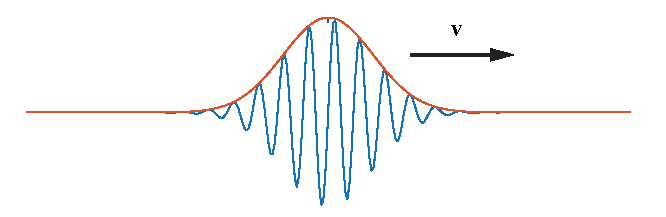
\includegraphics[width=12cm]{./figures/QM01.pdf}
\caption{蓝线是一维波函数/绳子的形状,橙线是振幅.某个位置的振幅越大,粒子就越有可能出现在该位置.图中的形状叫做波包,一般来说波函数可以是几乎任何形状.} \label{QM0_fig1}
\end{figure}

这里只讨论一维的情况,即粒子沿直线运动.经典力学中用位置关于时间的函数描述一个粒子的运动,而量子力学中用波函数描述.波函数是一个关于位置和时间的函数,例如一条紧绷的绳子(或弦)上的波动,绳子的高度 $y$ 是关于位置 $x$ 和时间 $t$ 的函数\footnote{波函数和绳子的运动方式相似但不完全相同}.某个位置震动的幅度的平方就是粒子在这个位置出现的概率\footnote{波函数的值是复数,粒子出现在某点的概率是复数模长的平方.这里为了简单暂时使用实数,可以看做是复数的实部}.经典力学中,给出粒子初始的位置和速度和势能,它将按照牛顿第二定律运动.量子力学中,给出粒子的初始波函数,波函数将按照含时薛定谔方程变化,把势能和某个时刻的波函数代入薛定谔方程,就可以解出任意时刻的波函数(这类方程并不是数的方程,而是函数的方程,所以解出的是函数,而不是数).薛定谔方程是量子力学的公设之一,就像牛顿三定律是牛顿力学的公设.量子力学中,粒子都用波表示,是因为许多实验发现微观粒子(如电子,质子,中子)具有一些波的性质,这就是著名的波粒二象性.

\subsection{波包}
即使粒子的位置一般不能精确确定,我们往往也能确定其大致范围(例如实验物理学家往往知道某粒子在实验室而不在月球),所以波函数往往只有在一定范围内不为零(我们只能在一定空间范围内测到检测到粒子).将振幅关于位置的函数画出来,其形状往往像一个包(越靠近中间,检测到粒子的概率越大),我们称为波包.

\subsection{自由粒子}

\begin{figure}[ht]
\centering
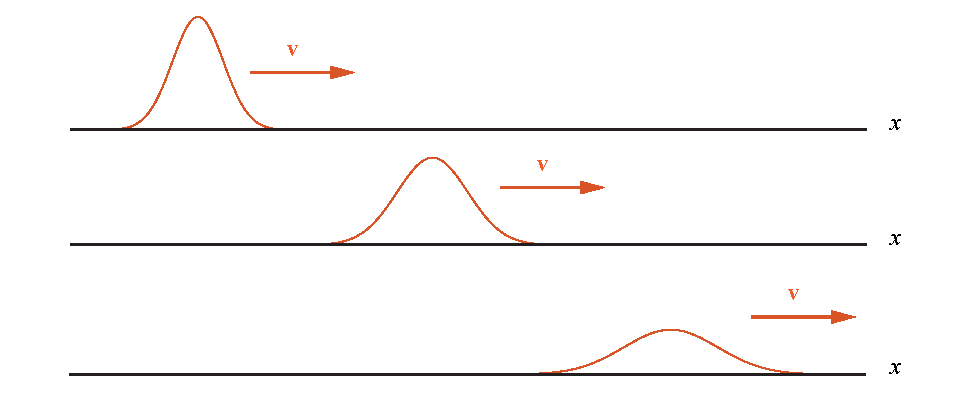
\includegraphics[width=14cm]{./figures/QM02.pdf}
\caption{对应自由粒子的波包.注意图中波包仅画出了振幅,没画出上一张图中的具体的波动形状.} \label{QM0_fig2}
\end{figure}

先看不受力的粒子(叫自由粒子),在经典力学中,粒子不受力时静止或者做匀速运动.量子力学中,若粒子不受力(势能处处为常数)且初始时波函数为波包且具有初速度,波包中心就会匀速运动,但同时波包会扩散(越变越宽,越变越矮).想象一根紧绷的绳子的一端突然迅速上下抖了几下又停下来,那么将产生一个波包将从绳的一段传到另一端(不同的是绳子上的波包形状不会变化).如果波包开始是静止,那么波包只会在原地扩散(这点与绳子的运动方式不同).

当我们回到宏观中,波包的大小就可以忽略不计, 把波包近似成质点,那波包的位置就是质点的位置,中心速度就是质点的速度\footnote{小时物理百科的 logo 就是自由高斯波包}.

\subsection{无限深势阱}
经典力学中,若质点在两面墙之间不停反弹,与墙不断发生完全弹性碰撞(碰撞后速度大小不变).如果用势能描述,就是墙之间的势能为零(或常数),墙和墙外的势能为无限大.这种势能叫做无限深势阱.量子力学中,波包在无限深势阱中同样一边来回碰撞一边扩散.

\subsection{散射}

\begin{figure}[ht]
\centering
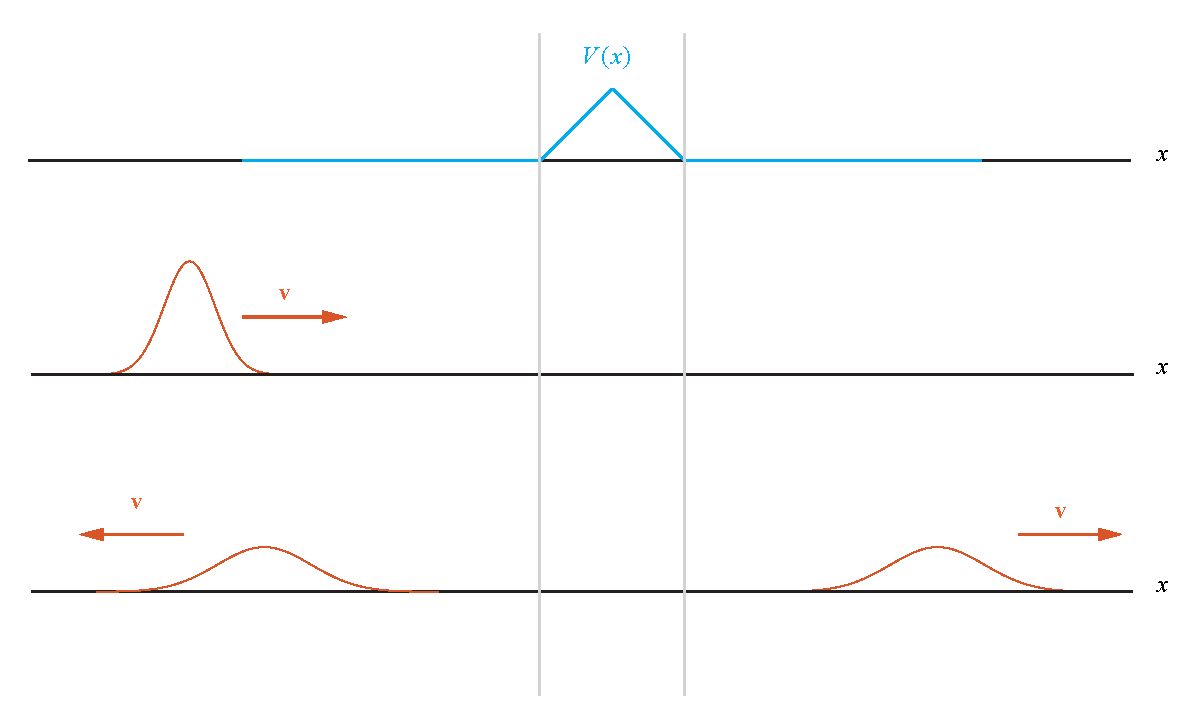
\includegraphics[width=14cm]{./figures/QM03.pdf}
\caption{波包遇到三角形势垒后的散射.} \label{QM0_fig3}
\end{figure}

经典力学中,若粒子匀速入射到如图所示的势能 $V(x)$(叫做势垒)上,如果粒子的初始动能小于势垒的最大值,则粒子将会原路返回,若粒子初始动能大于势垒的最大值,则粒子将继续前进.在量子力学中,无论波包以什么初速度入射,波包都会被分为两个不同方向运动的波包,但两个波包的相对大小取决于初始速度.

\subsection{波的叠加}
为什么要用波函数来描述粒子?因为波的一个重要特点就是可以叠加.如果一个波包是薛定谔方程的解,且另一个波包也是薛定谔方程的解,那这两个波包叠加(即把两个波函数相加)后仍然是薛定谔方程的解.例如:两个不同方向运动的波包相遇然后远离.注意这里两个波包并不代表两个粒子,而是代表一个粒子有可能在一个波包的位置被观测到也有可能在另一个被观测到.

\subsection{能量本征态}
在经典力学中,要测量一个粒子的能量,我们只需要先观测其速度,则能量等于动能($mv^2/2$)加上该位置的势能.量子力学中,测量波包的能量会得到什么结果呢?这时候我们需要薛定谔方程的另一个用途:对某个势能,我们能解出一些(往往是无穷多个)特殊的波函数,称为能量的\bb{本征函数}或者\bb{本征态}.如果粒子的波函数恰好是一个能量本征态,那么测量其能量会得到唯一确定的值(先不讨论用什么方法测)叫能量的本征值.每个本征态对应唯一一个本征值.

要测量任意波包(波函数)的能量,我们可以想办法用不同的能量本征态叠加来凑出所需波函数,例如第一个本征态乘以常数 $C_1$ 加上第二个本征态乘以常数 $C_2$ 等,这叫波函数的线性叠加.如果对这个波包测量能量,测到第 $i$ 个能量本征值的概率等于 $\abs{C_i}^2$ (之前提到波函数其实是复数,这里的系数事实上也同样是复数,而这里的绝对值符号代表复数的模长).也就是说,某个能量本征态占总波函数的比例越多,越有可能测出对应的能量本征值.

% 未完成:画出以上各例中能量本征态的图像.

\begin{figure}[ht]
\centering
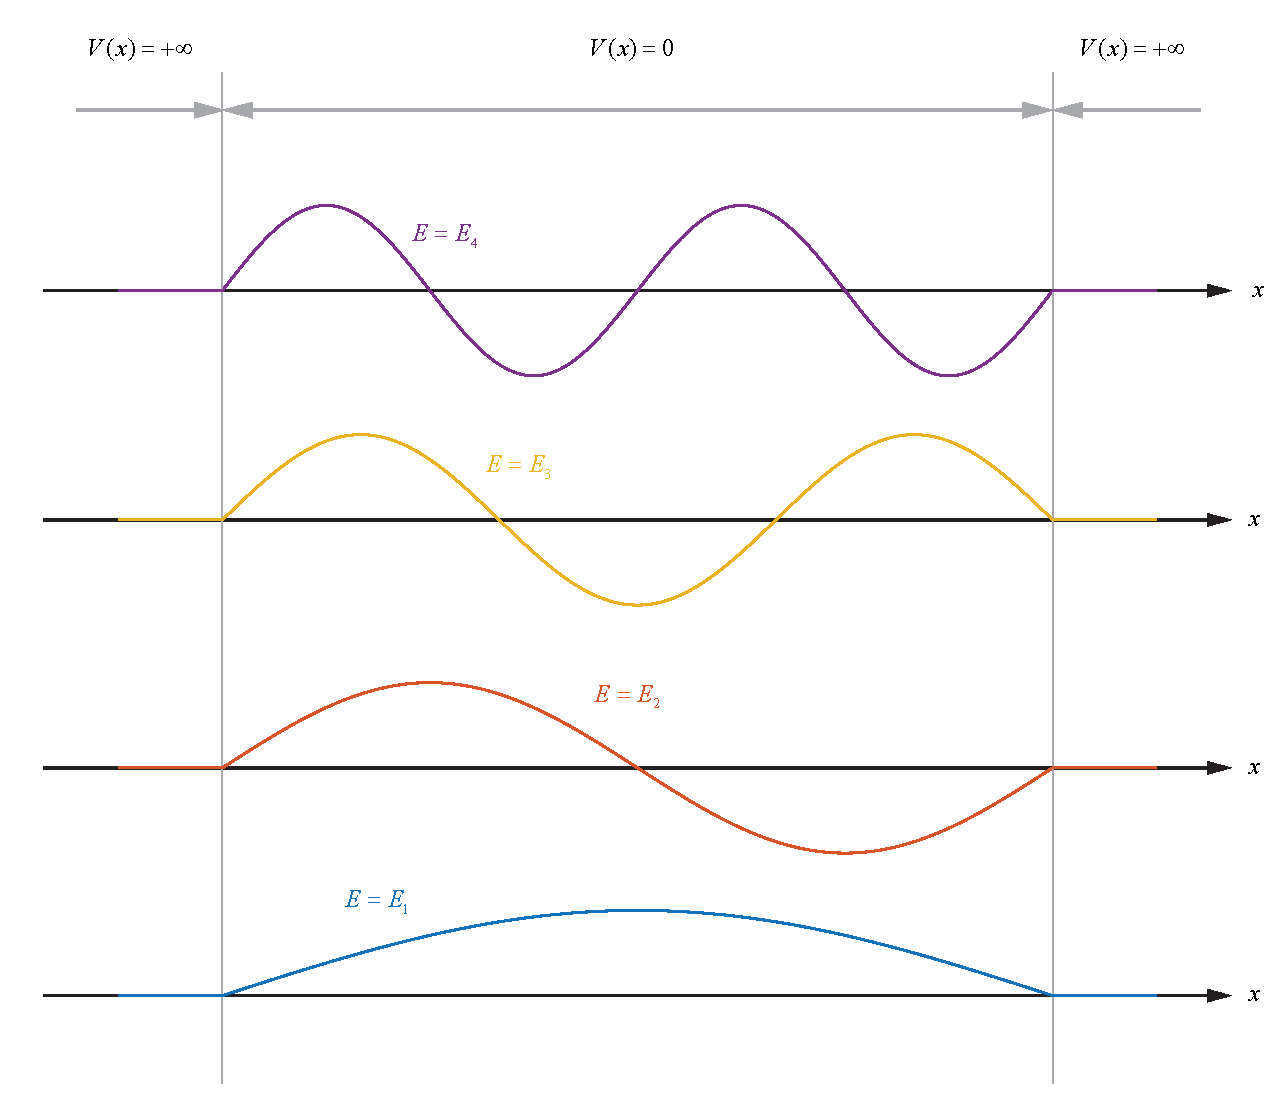
\includegraphics[width=14cm]{./figures/QM04.pdf}
\caption{无限深势阱的一些波函数能量本征态,每个能量 $E_i$ 叫做一个能级,共有无穷多个能级,将这些本征态叠加就能获得任何波函数例如波包.} \label{QM0_fig4}
\end{figure}

\subsection{测量理论}
我们介绍量子力学的另一个重要公设: \bb{测量理论}. 这里的\bb{测量}是一个抽象的概念, 我们不讨论用什么仪器进行测量,也不讨论现实中这种测量可不可行, 只是假设存在“ 测量某个物理量” 这种操作.

上面介绍的能量测量的步骤就是测量理论的一个特例. 量子力学中的任何物理量的测量都是由类似的方法求出, 只是求本征态的方法有所不同. 例如动量的本征态是一个无限长的波(某个频率的 $\sin$ 函数, 称为\bb{平面波}, 区别与波包), 位置的本征态是一个无穷窄的波包(称为 $\delta$ 函数), $\delta$ 函数描述的粒子只可能出现在某点. 如果要对一个粒子测量某物理量,就先计算出各个本征态占波包的比例 $C_i$,测量到第 $i$ 个本征值的可能性就是 $\abs{C_i}^2$.

这里有一个条件是任何物理上可能存在的波包都可以由任何测量量的本征态叠加而成,这叫做本征态的完备性.

在进行测量后, 如果得到第 $i$ 个本征值, 粒子的状态会立即\bb{坍缩}为这个本征值对应的本征态, 然后继续按照薛定谔方程演化.

那么我们应该如何理解测量到某个本征值的概率 $\abs{C_i}^2$ 呢? 这里显然不是指对处于某状态的粒子连续测量 $N$ 次, 就大概有 $\abs{C_i}^2 N$ 次会测到本征值. 因为只有第一次测量的概率是 $\abs{C_i}^2$ , 之后由于波函数会坍缩到第 $i$ 个本征态并继续按薛定谔方程继续演化, 再次测量时, 我们就要根据新的波函数重新计算每个 $C_i$, 而不是使用第一次测量前波函数.

正确的理解应该是, 如果我们有 $N$ 个处于同样状态(具有相同波函数)的相同粒子, 对这些粒子进行测量, 大概会有 $\abs{C_i}^2 N$ 个次测量得到第 $i$ 个本征值. 或者是, 我们把同一个粒子测量 $N$ 次, 但每次测量后都进行某种操作, 将其恢复到测量前的状态, 再进行下一次测量.

这就意味着, 除非粒子在测量前就已经处于该本征态, 测量操作必定会改变粒子的状态. 例如粒子的波函数如为\autoref{QM0_fig1} 中的波包, 当我们测量其位置, 如果得到的值为 $x_0$, 那么波函数将会马上变为 $x_0$ 处的一个无限窄的波包.

\subsection{连续本征值与离散本征值}
上面我们提到一个物理量往往有无穷多个本征波函数.一些情况下我们求出的本征波函数对应的值是不连续的(如无限深势阱中的能量本征态),而另一些情况下则是连续的(如动量的本征态总是连续的).经典物理世界中这些物理量都是连续的,而量子中的物理量会出现离散的情况. 这就是 “量子” 这个词的来源(表示一份一份的).

\subsection{薛定谔的猫}
注意我测量理论中并没有指明什么样的事件会构成测量. 还是用上面的例子, 假设一个粒子的波函数是两个反方向运动的波包, 且两个波包的形状相同. 我们在一个方向放一个屏幕用于测量位置, 检测到粒子后, 屏幕会发光. 那么根据测量理论, 这个粒子有 $1/2$ 的概率会落到屏幕上(朝着屏幕方向运动的波包). 按照通常的理解, 这似乎就对粒子构成了测量.

但是这并不严谨, 因为屏幕也是由微观粒子(质子,电子等)构成的, 也可以由波函数描述. 如果将屏幕与粒子作为考察的系统, 我们可以用一个多粒子的波函数来描述这整个系统(多粒子的波函数这里作不介绍). 当一个波包传播到屏幕的位置时, 波函数描述下的屏幕的也变为包含发光的本征态与不发光的本征态的叠加, 正如粒子的初始状态是向左传播的波函数和向右传播的波函数的叠加. 

如果假设“人眼看屏幕” 这个操作对屏幕的波函数进行了测量, 那么只有当实验者去看屏幕的瞬间, 波函数才会坍缩到屏幕发光或不发光的本征态.

这个论述可以一直进行下去, 人眼也是由微观粒子构成的, 那么如果也纳入考察的系统(用波函数描述), 那人眼的状态就会是“看到发光屏幕的人眼”和“没有看到发光屏幕” 的人眼这两种本征态的叠加, 直到人脑对人眼进行测量后才会得到确定的结果. 实验者最终也会处于“看到发光屏幕的人”和“没看到发光屏幕的人” 这两种本征态的叠加态.

\bb{薛定谔的猫}就是这类佯谬中的一个具体例子. 在这个假想实验中, 一瓶放射性物质旁边放有一个粒子检测器(改革计数器), 当检测器检测到放射性出的粒子时, 就会触发一个释放毒药的开关, 将箱子里的猫毒死. 由于放射出的粒子是由波函数描述的, 对这个实验的理解取决于这一系列过程中的哪一步构成测量. 如果我们认为检测器对放射粒子构成了测量, 那么从测量到结果的那一刻, 一切都是确定的, 也就不存在佯谬. 但如果我们认为只有当人打开箱子看到猫的那一刻才构成测量, 那么在打开箱子前猫都处于死和活两个本征态的叠加态. 更不可思议的理解是, 根本不存在测量, 当人打开箱子检查后, 人也成了“看到活猫” 的人和“看到死猫” 的人的叠加态.

关于什么构成测量这个问题至今仍然没有公认的解释, 但在现实中研究者往往假设测量仪器对粒子构成了测量\footnote{这一方面也是因为多粒子波函数的计算极其复杂的原因. 目前我们还无法计算多于两个粒子的波函数的薛定谔方程, 即使是用超级计算机做数值解。 量子力学中所有涉及多粒子波函数的理论几乎都是用了不同程度的近似。}, 且得到的实验与计算的高度吻合。

\subsection{不确定性原理}

\begin{figure}[ht]
\centering
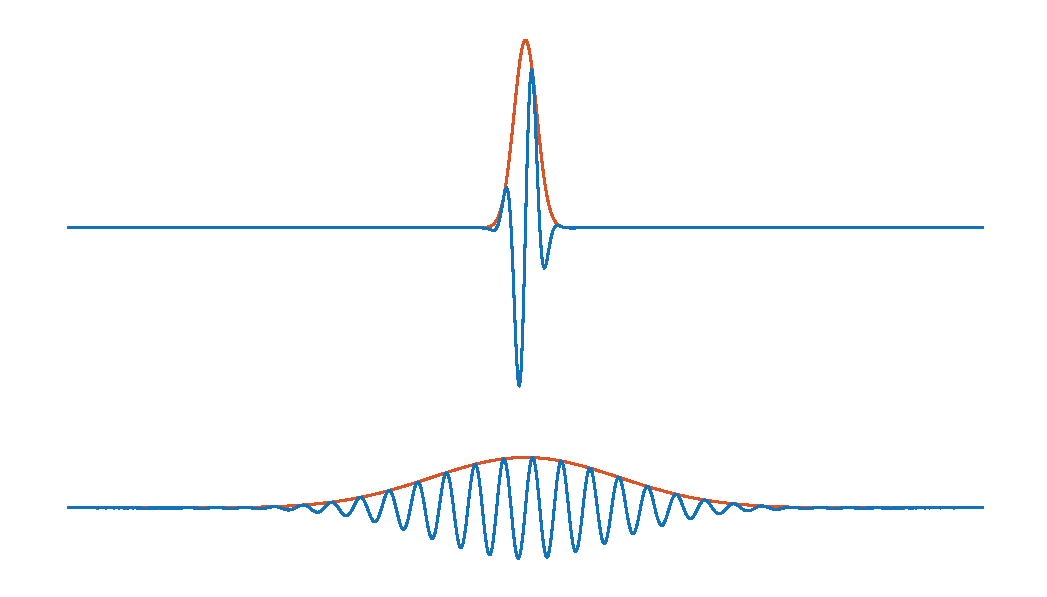
\includegraphics[width=14cm]{./figures/QM05.pdf}
\caption{波包越短,频率就变得越模糊,波包越长,频率就变得更精确.} \label{QM0_fig5}
\end{figure}

不确定性原理是说,我们无法既准确测量粒子的位置和动量.上文提到位置的本征态是一个无限窄的波包,对应本征值为该波包的位置(坐标).动量的本征态恰恰相反,是平面波.动量的征值为平面波的频率.

如果波包很窄(但不是无限窄),那么要测量位置,我们只需要使用波包中心附近的一些位置本征态就可以叠加出待测的波包,所以测量结果也只可能离波包中心较近.但在测量动量时,由于这个波包和平面波一点都不像,我们需要非常多的不同频率的平面波叠加才能得到这个波包(为什么无限长的平面波相加能得到有限长的波包?这是数学上一个非常有趣的结果,叫做傅里叶变换.)

另一种情况是,如果波包很长但不是无限长(想象绳子的一段连续上下抖了许多下才停下来),那么将波包看起来与某个频率的平面波十分相似.在测量位置时,我们需要将许多不同坐标的位置本征函数叠加得到波包,那测得的坐标就可能在很大的范围内出现.而测量动量时,我们只需要使用某个频率附近的一些平面波,所以测得的动量(与频率成正比)也都很接近中心频率对应的动量.

